% !TEX root = ../../../main.tex
% 来源：中学数学实验教材·第一册（代数）
% 章节：一元二次方程 / 平方与平方根
% 原始文件：3.tex，行 829-856
% 类型：tikz
% ---
 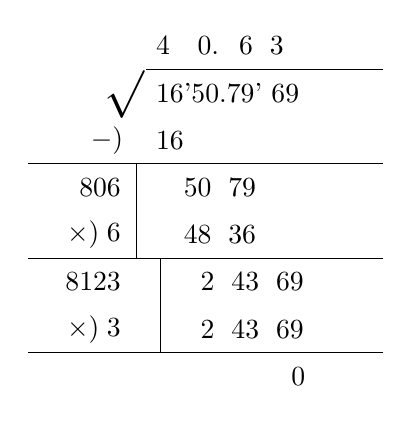
\begin{tikzpicture}[yscale=.6, >=latex]
    \node at (0,2)[right]{4\quad 0. \;6\; 3};
\node at (0,1)[right]{16'50.79' 69};  
\node at (0,0)[right]{16};    
\node  at (0,-1)[right]{\quad 50\; 79};     
\node at (.1,1)[left]{\LARGE $\sqrt{}$};
\node at (0,-2)[right]{\quad 48\; 36};  
\node   at (0,-3)[right]{\quad\; 2\; 43\; 69};
\node at (0,-4)[right]{\quad\; 2\; 43\; 69};
\node   at (0,-5)[right]{\qquad\qquad\;\; 0};
\draw(0,1.5)--(3,1.5);

\foreach \x in {-2.5,-4.5}
{
    \draw (-1.5,\x)--(3,\x);
    \draw (-0.5-\x*.15,\x)--(-0.5-\x*.15,\x+2);
}

\node at (-.5,0) {$-)$};

\draw (-1.5,-.5)--(3,-.5);
 
\foreach \x/\xtext in {-1/806 , -2/\times)\; 6  , -3/8123, -4/\times)\; 3 }
{
   \node at (-.2, \x)[left]{$\xtext$};
}

\end{tikzpicture}       
